% ----------------------------------------------------------
% Subseção Consciência
% ----------------------------------------------------------
\subsection{Consciência}
Um momento lógico pode ser formado por uma divisão (primeiro momento) ou por subdivisões lógicas (demais momentos).
	\begin{figure}[H]
	\caption{Intervalo lógico}
	\label{fig:consciousness_logical_moments}
	\centering
	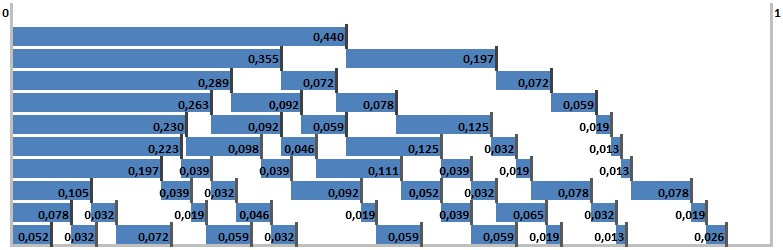
\includegraphics[scale=.7]{sections/images/consciousness_logical_moments.jpg}
	\floatfoot{Exemplo de um intervalo lógico com dez momentos lógicos.}%\footnotemark}
	\end{figure}
	%\footnotetext{Fonte: note}

A consciência são os momentos lógicos de uma expansão representados em suas unidades.
	\begin{figure}[H]
	\caption{Intervalo lógico consciente}
	\label{fig:consciousness}
	\centering
	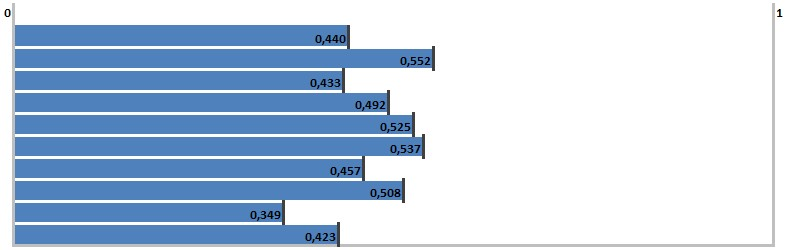
\includegraphics[scale=.7]{sections/images/consciousness.jpg}
	\floatfoot{Exemplo de um intervalo lógico consciente com dez unidades de momentos lógicos.}%\footnotemark}
	\end{figure}
	%\footnotetext{Fonte: note}

Pode ser observado na Tabela \ref{tab:10000_all} que a probabilidade de 99,99\% das amostras de uma população (Amostras do Range), que aumentam em quantidade à medida que crescem os momentos lógicos, tendem a estar cada vez mais ao centro do intervalo lógico, sendo que essa centralização tende ao infinito.
	\begin{figure}[H]
	\caption{Centralização de 99,99\% das amostras}
	\label{fig:centering_of_99_range}
	\centering
	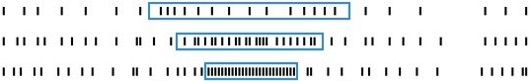
\includegraphics[scale=1]{sections/images/centering_of_99_range.jpg}
	\floatfoot{Tendência de centralização do range de 99,99\% das amostras.}%\footnotemark}
	\end{figure}
	%\footnotetext{Fonte: note}

A consciência tende à representação de uma onda lógica, a maior onda lógica de uma população, um histograma da distribuição normal, conforme Figura \ref{fig:trend_chart_of_normal_distribution}. Todos os aspectos listados abaixo são inerentes a abstração lógica chamada consciência.

\subsubsection{Infinito}
Um dos aspectos mais importantes que a negação do nada traz (negação de si), é o infinito, ou seja, em qualquer intervalo lógico cabe o infinito novamente. A lógica primordial que iniciou todo o intervalo lógico é a mesma encontrada em seus intervalos subsequentes. Isso fundamenta como uma lógica de alto nível como a subconsciência humana explica a lógica primordial, uma vez que não é preciso voltar ao primeiro momento lógico do intervalo para deduzi-lo, pois esse fenômeno é onipresente em todo o intervalo.

\subsubsection{Ondas}
Probabilisticamente a distribuição de novas amostras de uma população tendem a concentrar mais amostras sentido a mediana da população com frequências de amostras cada vez maiores neste sentido. Porém, a distribuição dessas amostras com frequências de crescimento uniformes é infinitesimal se comparado às possibilidades randômicas desse crescimento. Assim, a tendência de crescimento dessas frequências sentido a mediana somadas a baixíssima probabilidade (infinitesimal) desse crescimento ser uniforme, conduz a frequências no padrão de ondas. A relação de densidade ou amplitude de uma onda com seu comprimento é detalhada subseção posterior.
	\begin{figure}[H]
	\caption{Padrão de onda}
	\label{fig:consciousness_waves}
	\centering
	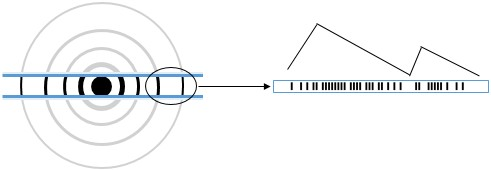
\includegraphics[scale=.8]{sections/images/consciousness_waves.jpg}
	\floatfoot{Padrão de onda inferido pela tendência dessa distribuição com frequências maiores sentido a mediana da população e a baixíssima probabilidade de crescimento uniforme dessas frequências.}%\footnotemark}
	\end{figure}
	%\footnotetext{Fonte: note}

A junção de uma onda a outra elimina sua discrepância e faz com que essa onda deixe de existir a se tornar parte da primeira, que tem seu pico mais próximo da mediana. Uma onda não morre, apenas une-se com outra onda mais ao centro da população.
	\begin{figure}[H]
	\caption{Unificação de ondas}
	\label{fig:consciousness_uniform_wave}
	\centering
	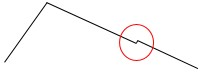
\includegraphics[scale=1]{sections/images/consciousness_uniform_wave.jpg}
	\floatfoot{Ondas sendo unificadas para exemplificar o crescimento amostral uniforme.}%\footnotemark}
	\end{figure}
	%\footnotetext{Fonte: note}

\subsubsubsection{Comprimento e amplitude}
O histograma é utilizado nas figuras dessa subseção e posteriormente para facilitar a visualização e entendimento, pois representa muito bem a curva de densidade de uma população, conforme as diferentes visualizações da Figura \ref{fig:consciousness_wave_histogram} representando apenas um intervalo ou um comprimento de onda pareado pela mediana da população.  
	\begin{figure}[H]
	\caption{Histograma em diferentes visualizações }
	\label{fig:consciousness_wave_histogram}
	\centering
	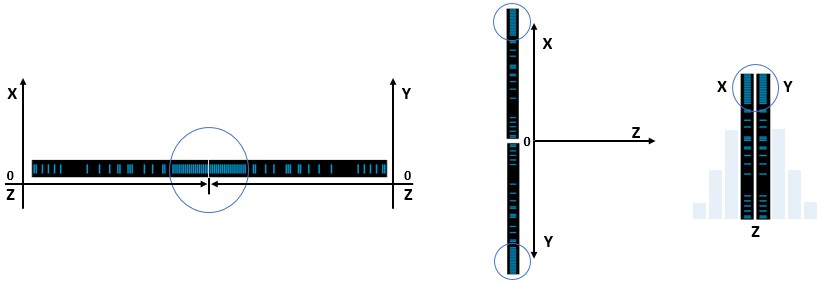
\includegraphics[scale=.7]{sections/images/consciousness_wave_histogram.jpg}
	\floatfoot{Diferentes maneiras da representação populacional em histograma.}%\footnotemark}
	\end{figure}
	%\footnotetext{Fonte: note}}
O comprimento e amplitude de ondas estabelecem uma relação de quantidade por intervalo ou unidade. Essas unidades são estabelecidas pelo entrelaçamento de ondas, conforme subseção posterior. Assim, a amplitude é a densidade de um comprimento de onda, a densidade de um intervalo qualquer.  

Ao adicionar uma nova amostra na população todo o intervalo se distribui proporcionalmente para acoplar essa amostra. Ao observar a população em intervalos ou comprimentos de ondas menores suas amplitudes de ondas obedecerão a distribuição de amostras desses subintervalos proporcionalmente, conforme Figura \ref{fig:consciousness_space_volume_amplitude}.
	\begin{figure}[H]
	\caption{Comprimento vs Amplitude de onda}
	\label{fig:consciousness_space_volume_amplitude}
	\centering
	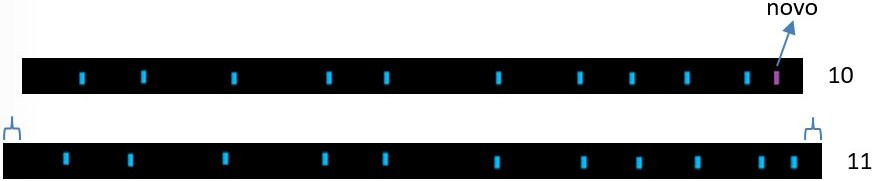
\includegraphics[scale=.4]{sections/images/consciousness_space_volume_amplitude.jpg}
	\floatfoot{Relação de comprimento e amplitude de ondas.}%\footnotemark}
	\end{figure}
	%\footnotetext{Fonte: note}}

Outro fator importante é que as novas amostras tendem a serem mais distribuídas no pico do intervalo, provavelmente o local mais denso da onda. Na da Figura \ref{fig:consciousness_space_amplitude_growth} o pico é representado na parte superior do subintervalo que compõe o pico da onda (porque é o intervalo mais denso que compõe o pico e porque a parte superior do intervalo está mais próxima de a mediana da população). No entanto, o pico pode estar em qualquer outro ponto nos subintervalos que compõem o pico de uma onda.
	\begin{figure}[H]
	\caption{Amplitude de onda - pico}
	\label{fig:consciousness_space_amplitude_growth}
	\centering
	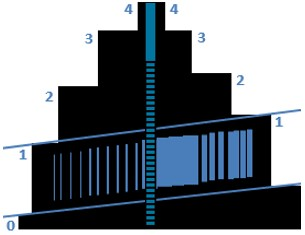
\includegraphics[scale=.6]{sections/images/consciousness_space_amplitude_growth.jpg}
	\floatfoot{Tendência da maior concentração de amostras nos subintervalos de uma onda maior.}%\footnotemark}
	\end{figure}
	%\footnotetext{Fonte: note}}

Em grandes intervalos com muitos momentos lógicos é observado uma discrepância menor das amplitudes das ondas. Nesses intervalos podem ser observados grandes sistemas de objetos. Quanto maiores os intervalos mais equilibrados eles estarão crescendo sentido a mediana da população, probabilisticamente, conforme Figura \ref{fig:consciousness_space_subconsciousness}. A onda mais inferior, azul escuro, é a onda base do sistema, ou seja, a onda que formou as outras ondas. Os sistemas de ondas podem ser complexos, tendo várias ondas aninhadas, melhor visto na Figura \ref{fig:consciousness_gravitational_force_system}. Intervalos mais complexos e com essa característica podem representar, por exemplo, o centro do universo, então o centro de uma galáxia, estrelas, planetas etc.
	\begin{figure}[H]
	\caption{Amplitude de ondas em grandes intervalos ou comprimentos}
	\label{fig:consciousness_space_subconsciousness}
	\centering
	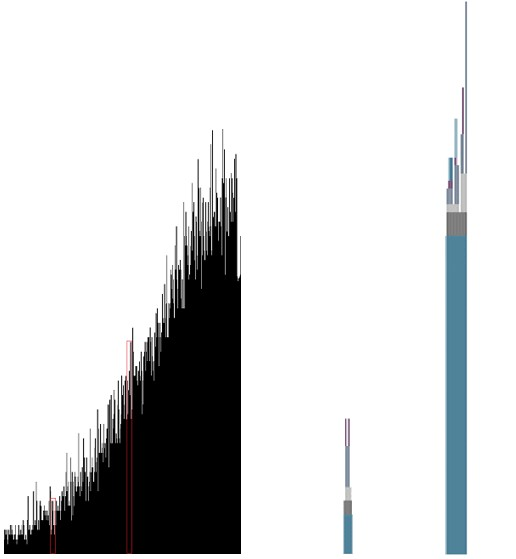
\includegraphics[scale=.45]{sections/images/consciousness_space_subconsciousness.jpg}
	\floatfoot{Menor discrepância das ondas em grandes intervalos.}%\footnotemark}
	\end{figure}
	%\footnotetext{Fonte: note}

Em intervalos menores e com muitos momentos lógicos é observado uma discrepância maior das amplitudes das ondas. Nesses intervalos podem ser observados sistemas menores de objetos. Quanto menores os intervalos mais desequilibrados eles estarão crescendo sentido a mediana da população, probabilisticamente, conforme Figura \ref{fig:consciousness_space_subconsciousness_min}. A onda mais inferior, azul escuro, é a onda base do sistema, ou seja, a onda formadora de outras ondas. Os sistemas de ondas mais complexos e com essa característica podem representar, por exemplo, o átomo que são muito pequenos, se apresentam em enormes quantidades e as partículas que orbitam seu núcleo (elétrons) ficam bem mais distantes dele.
	\begin{figure}[H]
	\caption{Amplitude de ondas em pequenos intervalos ou comprimentos}
	\label{fig:consciousness_space_subconsciousness_min}
	\centering
	
\includegraphics[scale=.45]{sections/images/consciousness_space_subconsciousness_min.jpg}
	\floatfoot{Alta discrepância das ondas em pequenos intervalos.}%\footnotemark}
	\end{figure}
	%\footnotetext{Fonte: note}}

\subsubsubsection{Entrelaçamento}
As amostras que mais se parecem em termos de frequências e distribuição são as amostras que fazem parte da mesma onda. Elas são frequências opostas não sobrepostas que se completam.

Probabilisticamente, as duas partes complementares de uma onda tendem a estar a uma distância aproximadamente iguais, equidistante da mediana, porém essa não é uma regra e as partes complementares de uma onda podem estar em distâncias diferentes em relação à mediana. O fenômeno da paridade das partes de uma onda tem o nome de entrelaçamento de ondas.

Esses pares tendem a serem formados pela probabilidade, onde comprimentos de ondas iguais detém a mesma probabilidade de distribuição de amostras em dois ou mais pontos diferentes da população. 

Intervalos com frequências temporais e distribuições espaciais parecidas são intervalos formados pela mesma unidade probabilística, ou seja, intervalos que têm o mesmo cenário ou contexto probabilístico em dado momento lógico. Por estarem no mesmo cenário probabilístico (unidades probabilísticas) esses intervalos têm suas amostras no mesmo cenário espaço-temporal, que é chamado de malha espaço-tempo e é formado pela maior unidade probabilística da população (todas as amostras da população intermediadas pela mediana). 

Esses entrelaçamentos formam ondas menores (subconsciências), semelhantes a maior onda do intervalo, comumente entrelaçada pela mediana da população, a consciência. A consciência é a lógica do intervalo, enquanto formam subconsciências ou sub-lógicas, como pequenas ondas de uma onda maior, sendo essas pequenas ondas semelhantes ao padrão da onda maior. Assim, uma mudança na onda maior (consciência) também é uma mudança na onda menor (subconsciência), mudança essa que é induzida pelas subconsciências indiretamente, análogo ao comprimir gás em um cilindro, onde ao adicionar uma nova molécula de gás no cilindro parcialmente cheio mais próximas ou apertas as moléculas dentro dele estarão. O contrário também é verdadeiro, uma nova amostra em uma subconsciência que por esta é observada diretamente é também uma mudança da consciência e vai ser induzida por outras subconsciências indiretamente, conforme Figura \ref{fig:consciousness_space_plan}.
	\begin{figure}[H]
	\caption{Subconsciência}
	\label{fig:consciousness_subconscious}
	\centering
	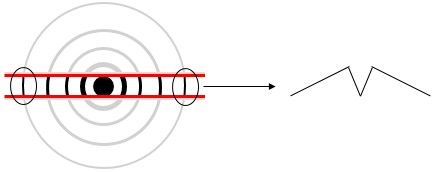
\includegraphics[scale=.8]{sections/images/consciousness_subconscious.jpg}
	\floatfoot{O padrão de ondas forma subconsciências semelhantes ao padrão criado pela consciência, como visto na Figura \ref{fig:trend_chart_of_normal_distribution}.}%\footnotemark}
	\end{figure}
	%\footnotetext{Fonte: note}
	
O entrelaçamento de ondas pode ocorrer em diferentes níveis ou intervalos, conforme visto na Figura \ref{fig:consciousness_subconscious_entanglement}, o que forma sistemas. As chavetas sem bordas (direita) identificam os intervalos os quais uma nova amostra despertou o salto, conforme visto na próxima subseção. Os arcos numerados indicam a ordem dos entrelaçamentos. Um entrelaçamento pode ocorrer de maneira equidistante da mediana não havendo o salto, como o primeiro entrelaçamento (violeta).

O maior entrelaçamento é mostrado nos exemplo da Figura \ref{fig:consciousness_subconscious_entanglement} como o primeiro entrelaçamento (violeta), ocorrido quando esse intervalo era o menor, provavelmente. Os grandes intervalos tendem a ser mantido ordenados pelas reordenações de seus subintervalos subsequentemente. A maior onda é comumente entrelaçada pela mediana da população. 

Os intervalos menores tendem a sofrer o entrelaçamento primeiro e essas reordenações causadas por eles permitem o entrelaçamento de pares com intervalos maiores. Os pares entrelaçados são os dois lados opostos de uma onda (pico ou vale) e se entrelaçam por sua mediana, que pode coincidir com a mediana da população quando se trata da maior onda probabilística.
	\begin{figure}[H]
	\caption{Níveis do entrelaçamento de ondas - comprimentos de ondas}
	\label{fig:consciousness_subconscious_entanglement}
	\centering
	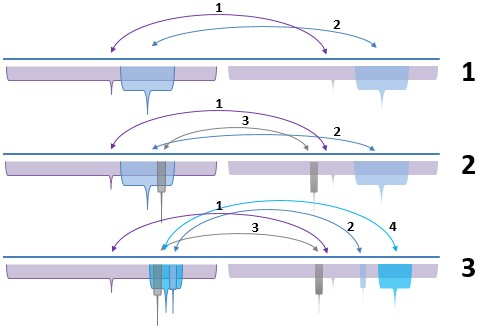
\includegraphics[scale=.8]{sections/images/consciousness_subconscious_entanglement.jpg}
	\floatfoot{Exemplos dos níveis do entrelaçamento de ondas ou níveis dos comprimentos de ondas.}%\footnotemark}
	\end{figure}
	%\footnotetext{Fonte: note}

Os possíveis comprimentos de ondas de uma população são definidos por esses níveis de entrelaçamentos de ondas. Assim, independente da ordem dos saltos, níveis maiores de entrelaçamento são os comprimentos de ondas maiores e níveis menores os comprimentos menores, o que permite que ondas maiores tenham sub-ondas menores. 

Todo entrelaçamento é uma onda e o encontro de dois entrelaçamentos não acarreta um novo entrelaçamento, apenas a soma dessas ondas, pois estas já estão entrelaçadas.  

O entrelaçamento ocorre em intervalos bem. Uma vez entrelaçados, cada nova amostra pode causar movimento, a depender do ambiente mais ou menos rarefeito. Os intervalos maiores são formados por meio da soma de intervalos menores já entrelaçados através do movimento e pela adição de novas amostras.

\subsubsubsection{Salto}
O salto é uma reordenação feita pelo entrelaçamento de ondas à medida em que as amostras dos pares entrelaçados deixam de ser equivalentes com a adição de novas amostras em um dos lados do par. O salto ocorre em uma das partes do par de uma onda e é uma reordenação, ou seja, tanto a parte do intervalo que acabou de receber a nova amostra deve melhor se adequar ao intervalo pretendido ao salto quanto o contrário.

Na Figura \ref{fig:consciousness_space_subconscious_observation_jump} é observado os entrelaçamento de ondas (representadas por colunas de um histograma para facilitar a visualização do intervalo). A reordenação feita pelo entrelaçamento provoca um salto nas coordenadas (X, Y e Z) conforme subseção do Espaço.
	\begin{figure}[H]
	\caption{Reordenação - Salto}
	\label{fig:consciousness_space_subconscious_observation_jump}
	\centering
	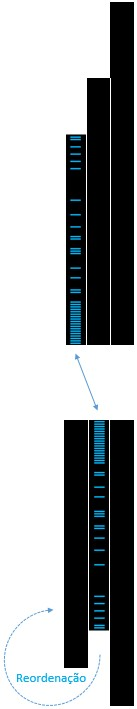
\includegraphics[scale=.53]{sections/images/consciousness_space_subconscious_observation_jump.jpg}
	\floatfoot{Salto provocado pela não equivalência do par entrelaçado com a adição de novas em um de seus lados.}%\footnotemark}
	\end{figure}
	%\footnotetext{Fonte: note}

Como exemplo, um fóton ao entrar no intervalo do elétron pode desequilibrar um dos lados do par entrelaçado do elétron que o faz saltar, porém como o intervalo do elétron é pequeno e o fóton é rápido (por ser ainda menor) ele sai rapidamente do intervalo do elétron que fica desequilibrado novamente e retorna para o nível de energia equivalente ao anterior ao salto.

\subsubsection{Tempo}
O tempo é a adição de novos momento lógicos entre momentos existentes à medida que prossegue a negação de si da lógica. Essas mudanças são acumulativas e a medida que aumentam o número desses momentos lógicos, menos relevante cada novo momento será dentro do intervalo consciente. Um em cem é mais relevante do que um em mil. 
	\begin{figure}[H]
	\caption{Tempo}
	\label{fig:consciousness_time}
	\centering
	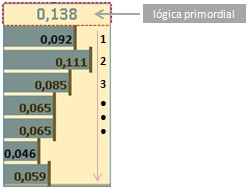
\includegraphics[scale=.8]{sections/images/consciousness_time.jpg}
	\floatfoot{Progressão do tempo conforme os momentos lógicos avançam.}%\footnotemark}
	\end{figure}
	%\footnotetext{Fonte: note}

Na introdução desse artigo foi apresentado que a lógica é uma sequência de negações de si no tempo zero, ou seja, em nenhum momento entre suas negações a lógica passa a \underline{SER}, garantindo a premissa primordial da constante lógica, \underline{NÃO SER}. Assim, a lógica é uma sequência infinita, simultânea e generalizada, uma constante. Na experiência do tempo conduzida pelo observador a ordenação da sequência é a essência dessa grandeza e, portanto, mais relevante do que sua origem que é de natureza simultânea, o qual transcende o tempo.

Cada população tem uma ordem diferente em sua sequência e é essa ordem que dá origem à grandeza que chamamos de tempo. É essa ordem do universo ou da consciência que vai dar a noção do que acontece antes ou depois, ou seja, o passado, o presente e as prospecções futuras.

Outro fator importante ao observar o tempo (o observador é mais detalhado na subseção da consciência – Observador e a vida) é que, probabilisticamente, subconsciências ou intervalos mais próximos da mediana da população terão uma adição maior de novas amostras em seus intervalos, o que são observados diretamente por essas subconsciências. Por outro lado, subconsciências distantes da mediana da população terão uma adição menor de amostras em seus intervalos e sujeitam-se a um número maior de mudança induzidas indiretamente, conforme Figura \ref{fig:consciousness_subconscious}. Esse fenômeno de observação temporal proporcionado pela probabilidade de distribuição da população evita o paradoxo dos gêmeos \cite{brasilescola_paradoxo_gemeos}.

As prospecções de futuro do observador fundamentam-se na probabilidade de distribuição da população e, portanto, da distribuição probabilística de cada subintervalo dela. Logo, o universo tende a ser probabilístico ainda que aleatório em níveis de detalhes, o que faz os eventos serem inusitados ainda que preditos em algum nível, conforme as Figuras \ref{fig:consciousness_logical_moments} e \ref{fig:consciousness}. 

\subsubsection{Espaço}
Na Figura \ref{fig:consciousness_space_waves}, é exibida a densidade de amostras de uma população, onde os pares que tendem a mesma distribuição probabilística são colocados lado a lodo e representados em forma de histograma. A formação desses pares é proveniente do entrelaçamento de ondas.
	\begin{figure}[H]
	\caption{Pares entrelaçados representados em três dimensões espaciais}
	\label{fig:consciousness_space_waves}
	\centering
	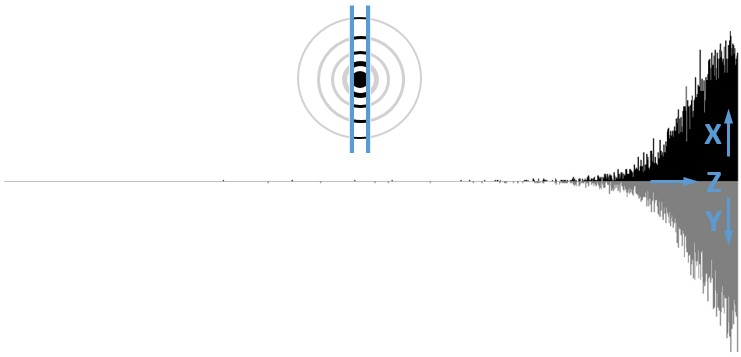
\includegraphics[scale=.7]{sections/images/consciousness_space_waves.jpg}
	\floatfoot{Exemplo de ondas entrelaçadas, representadas em forma de histograma e obtidas pelo algoritmo Logic\_WavePattern. \footnotemark}
	\end{figure}
	\footnotetext{O algoritmo Logic\_WavePattern pode ser visto no Apêndice \ref{app:algoritmos}.}

A área cresce de forma quadrática ao crescimento da amplitude de uma onda (colunas do histograma), uma vez que o salto provocado pelo entrelaçamento de ondas e a própria distribuição probabilística das amostras do intervalo tendem a manter um crescimento equivalente nos pares que formam uma onda. E esse aspecto configura a lei do inverso do quadrado, que será mais aprofundada na subseção da Força gravitacional.

Ao representar as grandezas espaciais do gráfico da Figura \ref{fig:consciousness_space_waves} em um gráfico de distribuição 3D e distribuir seus pontos de extremidade (desprezando seus volumes e possíveis pontos internos), obtém-se algo parecido com uma espiral (como redemoinhos no ar ou na água) mesmo em volumes muito pequenos de dados (poucos momentos lógicos), conforme Figuras \ref{fig:consciousness_space_3DScatter15000-10} e \ref{fig:consciousness_space_3DScatter_200000-2}. Os pontos tendem a se moverem em forma de espiral, aproximadamente, conforme mostra a subseção posterior. 
	\begin{figure}[H]
	\centering
		\begin{subfigure}[H]{0.47\linewidth}
		\centering
		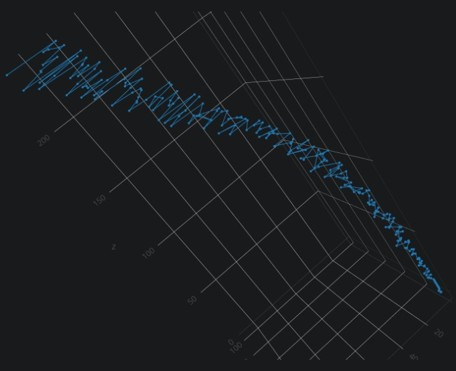
\includegraphics[width=1\linewidth]{sections/images/consciousness_space_3DScatter15000-10.jpg}
		\caption{15.000 amostras ou momentos}
		\label{fig:consciousness_space_3DScatter15000-10}
		\end{subfigure}
	
		\begin{subfigure}[H]{0.47\linewidth}
		\centering
		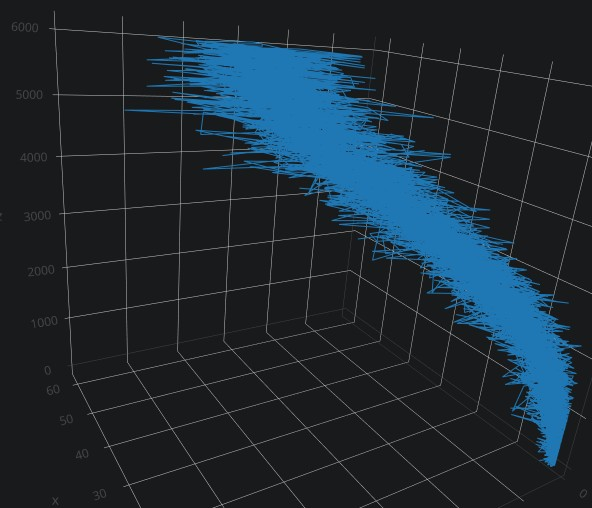
\includegraphics[width=1\linewidth]{sections/images/consciousness_space_3DScatter_200000-2.jpg}
		\caption{200.000 amostras ou momentos}
		\label{fig:consciousness_space_3DScatter_200000-2}
		\end{subfigure}%
	\caption{Gráficos de dispersão 3D gerados com pontos semelhantes aos da Figura \ref{fig:consciousness_space_waves}}
	\floatfoot{O histograma no padrão de ondas e os dados para gerar os gráficos de dispersão 3D podem ser obtidos com a execução do algoritimo Logic\_WavePattern. \protect\footnotemark}
	\end{figure}
	\footnotetext{O algoritmo Logic\_WavePattern pode ser visto no Apêndice \ref{app:algoritmos} e os gráficos de dispersão 3D podem ser acessados em: \url{https://chart-studio.plot.ly/create/?fid=ren.stuchi:5&fid=ren.stuchi:4} e \url{https://chart-studio.plot.ly/create/?fid=ren.stuchi:7&fid=ren.stuchi:6}}

Probabilisticamente, a grande concentração das amostras de uma população está em seu pico, sentido a mediana da população. Assim, devido à altas concentrações probabilísticas de amostras em intervalos cada vez menores de uma onda, o pico irá ocupar um subintervalo proporcional cada vez menor dentro da população, conforme observado na Figura \ref{fig:consciousness_flat_universe}. A figura \ref{fig:total_comparison_chart_with_99_range} é baseada na Tabela \ref{tab:10000_all} e também demonstra esta característica, que dentro da população pode demonstrar um universo aproximadamente homogêneo e plano na sua distribuição ainda que suas amostras tendam à linha de referência.  
	\begin{figure}[H]
	\caption{Universo plano}
	\label{fig:consciousness_flat_universe}
	\centering
	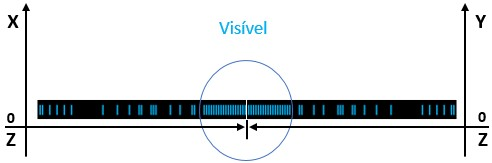
\includegraphics[scale=.6]{sections/images/consciousness_flat_universe.jpg}
	\floatfoot{Concentração de 99\% das amostras.}%\footnotemark}
	\end{figure}
	%\footnotetext{Fonte: note}

\textbf{Obviamente a representação e os movimentos do intervalo ou seus subintervalos entrelaçados não podem ser representados fielmente em 1 ou 2 dimensões, pois o entrelaçamento é essência inerente (inseparável) das 3 dimensões.} 

Cada nova amostra é tempo e também espaço (movimento ou mudança). Cada nova amostra adicionada dentro de um subintervalo fará este se movimentar conforme a distribuição de suas novas amostras. O intervalo ou seus subintervalos podem se movimentar em qualquer direção, porém da mesma forma que em uma distribuição em um 1D (eixo Z da Figura \ref{fig:consciousness_space_plan}) as amostras são concentras na parte de maior valor do plano, em 2D ou 3D é análogo e ocorre o mesmo, conforme exibido no subintervalo da Figura \ref{fig:consciousness_space_plan}. Tanto o intervalo quanto os subintervalos têm suas maiores concentrações de amostras sentido a sua linha de referência interna e das linhas de referências dos seus intervalos superiores. Isso faz com que algo aproximado com a representação dos histogramas vá se formando naturalmente. O intervalo e seus subintervalos têm seus tamanhos em X, Y e Z proporcionais a seus tamanhos dentro da população em representação 1D (eixo Z da Figura \ref{fig:consciousness_space_plan}), logo suas escalas internas estão relacionadas com a quantidade de amostras que eles têm.
	\begin{figure}[H]
	\caption{Distribuição espacial e movimento}
	\label{fig:consciousness_space_plan}
	\centering
	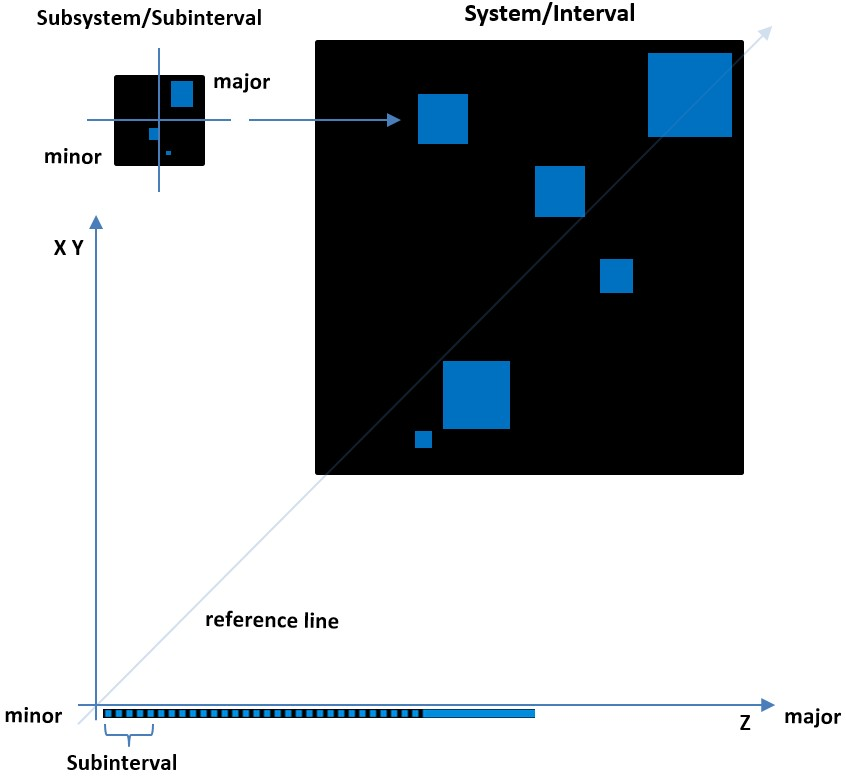
\includegraphics[scale=.6]{sections/images/consciousness_space_plan.jpg}
	\floatfoot{Distribuição espacial e movimento dos subintervalos e do intervalo populacional.}%\footnotemark}
	\end{figure}
	%\footnotetext{Fonte: note}
	
Uma nova amostra em um subintervalo movimenta este e seus intervalos superiores, pois uma mudança em um subintervalo também é uma mudança em seus intervalos superiores. O movimento é continuo e suas escalas de tempo e espaço são referentes a unidade básica da população (1 amostra [espaço] a cada nova amostra da população [tempo]). Por exemplo, um subintervalo pode estar se movimentando em uma direção a 2 amostra (espaço) a cada nova amostra da população (tempo) e continuará nesse movimento até que receba duas amostras internas contrárias ou trombe com alguma amostra em seu movimento, em ambientes mais ou menos rarefeitos, que diminua sua velocidade ou o faça parar (leis da dinâmica). 

O entrelaçamento ocorre em intervalos bem pequenos e eles se formam na base de seus intervalos superiores, de acordo com o eixo Z. Uma vez entrelaçados, cada nova amostra pode causar movimento, a depender do ambiente mais ou menos rarefeito. Os intervalos maiores são formados por meio da soma de intervalos menores já entrelaçados através do movimento e pela adição de novas amostras, conforme subseção do Entrelaçamento. Assim os movimentos dos elétrons dentro átomo não é totalmente continuo, pois, os saltos causam novos entrelaçamentos que redefine suas posições, configurando camadas.

Um subintervalo pode sair naturalmente da gravitação de seu intervalo superior. Isso ocorre mais facilmente com intervalos bem pequenos e rápidos (muitas amostras concentradas em um pequeno intervalo - pico) favorecido por seu movimento num ambiente rarefeito devido ao tamanho. 

É muito difícil saber a posição do intervalo ou de um subintervalo olhando para uma representação em 1D, pois cada nova amostra movimenta o subintervalo e o intervalo e essa interação requer um cálculo para representação que levaria até uma representação naturalmente em 3D novamente.

Todo subintervalo ao ser entrelaçado surge na base de seu intervalo superior. Logo, a adição de novas amostras nesse subintervalo que acabou de surgir o fará subir no seu intervalo superior e esse é o sentido de todos os entrelaçamentos, subir à medida que somam amostras e velocidade sentido a linha de referência. Porém o ambiente pode não rarefeito o que dificulta esse movimento (podendo o manter parado a depender do quão denso é esse ambiente). Outro fator que subtrai amostras de um intervalo é quando um de seus subintervalos recebe um salto e um novo entrelaçamento é definido, redefinindo a posição desse subintervalo na base de seu intervalo superior, o que subtrai deste os valores outrora somados em sua movimentação. Assim, na Figura \ref{fig:consciousness_space_plan_nosubinterval} é exibido um intervalo que ainda não contém subintervalos, portanto, ele sobe e ganha velocidade a cada nova amostra que ele recebe e sua subida vai ser centralizada se suas amostras são distribuídas uniformemente ou com um pico centralizado, ou será inclinada para a direita ou esquerda à medida que a concentração maior de amostras estiver mais de um lado do que do outro (é mais comum que a concentração de amostras esteja sentido a mediana da população).
	\begin{figure}[H]
	\caption{Intervalo sem subintervalos}
	\label{fig:consciousness_space_plan_nosubinterval}
	\centering
	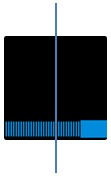
\includegraphics[scale=.7]{sections/images/consciousness_space_plan_nosubinterval.jpg}
	\floatfoot{Movimentação de um intervalo sem subintervalos.}%\footnotemark}
	\end{figure}
	%\footnotetext{Fonte: note}

\subsubsubsection{Espiral}
Como as coordenadas X, Y e Z dos pares emaranhados de uma população tendem a aumentar, a disposição dessas em um sistema tridimensional de coordenadas vai seguir uma referência diagonal entre esses três eixos, conforme Figura \ref{fig:consciousness_space_spiral_reference_line}. O padrão de espiral observado não invalida outros possíveis movimentos no espaço. Muitas vezes não é possível observar o padrão de espiral imediatamente nos movimentos de um intervalo (subconjunto), porém esse padrão está por traz de muitos destes movimentos. Ao pegar os movimentos humanos, como exemplo, tem-se os ciclos predominantes de ir e voltar para casa, ir e voltar ao trabalho, acordar e dormir, ou seja, os hábitos se assemelham a movimentos em ciclos, movimentos espirais.
	\begin{figure}[H]
	\caption{Sistema tridimensional de coordenadas}
	\label{fig:consciousness_space_spiral_reference_line}
	\centering
	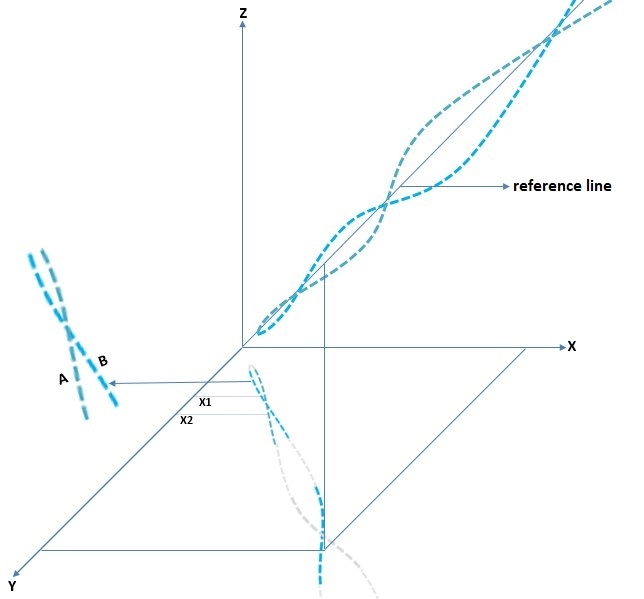
\includegraphics[scale=.7]{sections/images/consciousness_space_spiral_reference_line.jpg}
	\floatfoot{Linha de referência probabilística para distribuição de uma população em um plano tridimensional.}%\footnotemark}
	\end{figure}
	%\footnotetext{Fonte: note}}

Na Figura \ref{fig:consciousness_space_spiral_reference_line} também podem ser observado os pontos X1 e X2. Esses pontos foram espelhados nas coordenadas X e Z para facilitar a observação de que ao elevar o eixo Z também se eleva o eixo X ou Y, independente de seus pontos probabilísticos mínimos. A linhas tracejadas mostram os caminhos mais prováveis para os intervalos A e B. Dessa forma, quando uma parte do intervalo está em seu ponto médio máximo (eixos X e/ou Y) a tendência probabilística é que ele receba menos amostras do que a parte do intervalo que está em seu ponto médio mínimo. Esse efeito espiral é mais notável quanto maior for um intervalo e sua quantidade de amostras, pois mais prováveis e estáveis serão esses caminhos.

Cada intervalo ou subintervalo (comprimento de ondas) tem sua própria linha de referência. Assim como dentro de um metro existem os centímetros, milímetros etc., dentro de um intervalo e subintervalos podem existir inúmeros outros, conforme exibido abaixo e também na Figura \ref{fig:consciousness_gravitational_force_system}.
	\begin{figure}[H]
	\caption{Intervalos e linhas de referências}
	\label{fig:consciousness_space_spiral_underlines}
	\centering
	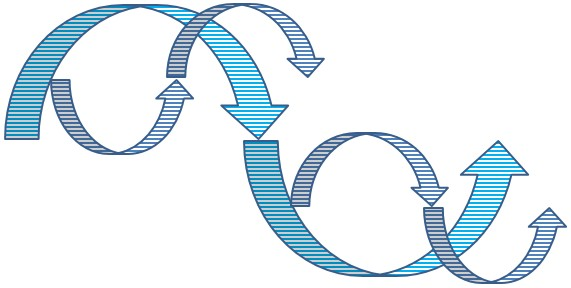
\includegraphics[scale=.5]{sections/images/consciousness_space_spiral_underlines.jpg}
	\floatfoot{Espirais em diferentes intervalos e suas linhas de referências.}%\footnotemark}
	\end{figure}
	%\footnotetext{Fonte: note}}

\subsubsection{Forças fundamentais}
A força gravitacional, a força eletromagnética e a força nuclear correspondem às chamadas forças fundamentais da natureza. Essas forças fundamentais não são forças propriamente, mas sim aspectos probabilísticos de distribuição da população e do entrelaçamento de ondas.

\subsubsubsection{Força gravitacional}
A força gravitacional não é uma força propriamente e sim um aspecto da probabilidade de distribuição de novas amostras sentido a mediana da população, conforme teorema central do limite. E sentido probabilístico faz com que as ondas tenham um caminho provável a seguir dentro da população, ou seja, o pico de amostras da população ou o pico da maior onda da população, conforme Figuras \ref{fig:consciousness_space_spiral_reference_line} e \ref{fig:consciousness_space_spiral_underlines}. Da mesma maneira, fazem também com que as amostras dentro de um intervalo tenham um caminho provável a seguir, ou seja, o pico de amostras do intervalo ou o pico da onda. Estes picos de amostras costumam ser a parte mais facilmente observáveis no intervalo de amostras desde ocupem uma área não tão pequena.

Na Figura \ref{fig:consciousness_gravitational_force} pode ser visto que a parte mais facilmente observável está levemente a direita no pico da onda. Essa onda tende a caminhar para cima e para direita, em uma diagonal que depende da distribuição probabilística das novas amostras, conforme mostrado pela maior quantidade de colunas azuis a direita da onda (sentido à mediana) em relação à esquerda.
	\begin{figure}[H]
	\caption{Força gravitacional}
	\label{fig:consciousness_gravitational_force}
	\centering
	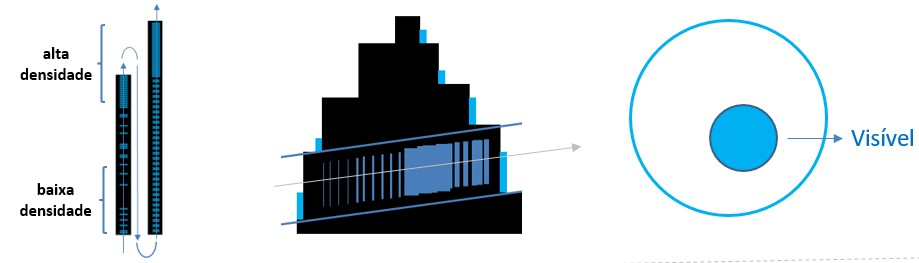
\includegraphics[scale=.7]{sections/images/consciousness_gravitational_force.jpg}
	\floatfoot{Aspecto gravitacional, o sentido probabilístico da distribuição de novas amostras dentro de um intervalo.}%\footnotemark}
	\end{figure}
	%\footnotetext{Fonte: note}

Conforme visto na subseção de Amplitude de ondas, a área de um intervalo cresce de forma quadrática, uma vez que o salto provocado pelo entrelaçamento de ondas e a própria distribuição probabilística das amostras tendem a manter um crescimento equivalente nos pares que formam a onda. Esse aspecto configura a lei do inverso do quadrado, onde, no caso da gravidade, quando mais perto os objetos, maiores serão as chances probabilísticas das novas amostras do objeto menor ir em direção ao objeto maior (o pico da onda), que por estar dentro de uma área quadrada menor e por consequência de menor possibilidades de posicionamento das amostras, as chances desses objetos se aproximarem com uma quantidade bem menor de momentos lógicos aumenta muito. Assim, quanto mais longe os objetos, maior a área, maior as possibilidades de posicionamento e mais momentos lógicos são precisos para a aproximação, caracterizando assim uma atração menor. A probabilidade também pode afastar objetos mais rarefeitos que devem estar mais afastados da parte mais facilmente observável e densa de amostras, como no caso do gás hélio, por exemplo. A distribuição de novas amostras nos intervalos rarefeito são mais lentas (caso contrário não seriam rarefeito) do que nas partículas mais densas que tomam a frete dessas partículas menos densas afastando-as do pico da onda. 

Quando observado todo o intervalo populacional, a onda mais inferior é a onda base de todas as outras sub-ondas, tendo a população uma quantidade expressiva de amostras. Desta mesma forma, ondas de níveis superiores, como as de nível dois da Figura \ref{fig:consciousness_gravitational_force_system} estão aninhadas em uma onda de nível um. Esses sistemas podem se tornar bem mais complexos em seus aninhamentos e são muito comuns. As linhas azuis na Figura abaixo representam as linhas de referências probabilísticas como explicado na Figura \ref{fig:consciousness_space_spiral_underlines}.
	\begin{figure}[H]
	\caption{Força gravitacional - sistema}
	\label{fig:consciousness_gravitational_force_system}
	\centering
	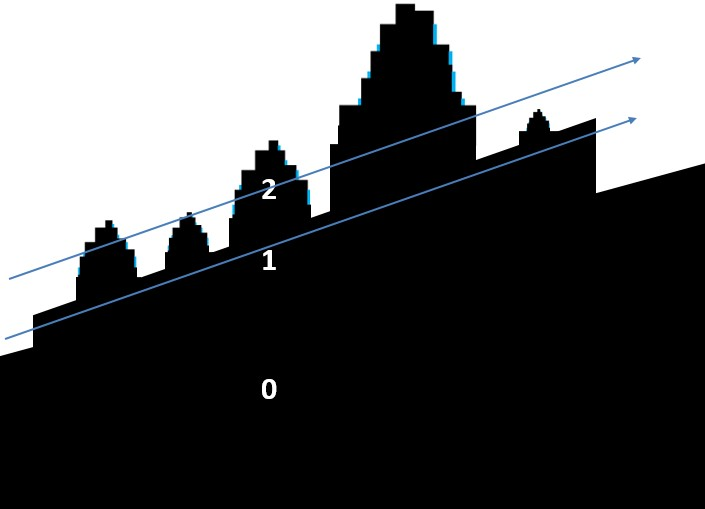
\includegraphics[scale=.5]{sections/images/consciousness_gravitational_force_system.jpg}
	\floatfoot{Aspectos gravitacionais de um sistema – onda base e suas sub-ondas.}%\footnotemark}
	\end{figure}
	%\footnotetext{Fonte: note}
	
A Figura \ref{fig:consciousness_gravitational_orbit} mostra em seu primeiro exemplo que a onda um, podendo ser um satélite, poderia se aproximar rapidamente da onda zero à medida que novas amostras vão sendo distribuídas dentro de todo o intervalo. O segundo exemplo mostra que a impulsão que o satélite recebe ao ser colocado em órbita faz com que sua onda tenha uma distribuição probabilística mais uniforme (esse crescimento uniforme é facilitado pela baixa densidade ao redor do pico probabilístico – 1 amostra em 100 é mais relevante do que 1 amostra em 1000), onde a parte da onda em azul está mais próxima da mediana da população e tem um crescimento ou deslocamento equivalente à sua onda inferior, o que a mantém constante. O terceiro exemplo é uma melhor visualização do segundo exemplo, para facilitar o entendimento, onde a onda um é definida pela espiral em torno do objeto circular que representa o pico probabilístico. Talvez a onda mais uniforme provocada pela impulsão (velocidade) possa facilitar o entendimento do adiantamento dos relógios atómicos nos satélites. Com este exemplo também fica mais fácil observar que a velocidade da luz não é constante, o que ocorre é que a onda de luz é tão menor que a parte da onda que fornece a velocidade é rapidamente desfeita, tornando-a praticamente constante.
	\begin{figure}[H]
	\caption{Força gravitacional - órbita}
	\label{fig:consciousness_gravitational_orbit}
	\centering
	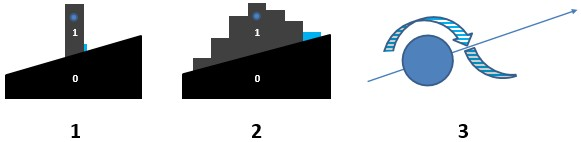
\includegraphics[scale=.9]{sections/images/consciousness_gravitational_orbit.jpg}
	\floatfoot{Aspectos gravitacionais de um sistema – órbita.}%\footnotemark}
	\end{figure}
	%\footnotetext{Fonte: note}	

\subsubsubsection{Força eletromagnética}
A força eletromagnética não é uma força propriamente e sim um aspecto do entrelaçamento de ondas que se intensifica em intervalos ou comprimentos de ondas com baixa entropia e com a aproximação espacial (redução de diferenças nos eixos X, Y e Z) desses intervalos.

O eletromagnetismo está relacionado à intervalos semelhantes a onda mais uniforme encontrada no segundo exemplo da Figura \ref{fig:consciousness_gravitational_orbit}, porém com baixa entropia, ou seja, a mesma estrutura que facilita o movimento dos objetos somado a baixa entropia, a qual facilita os saltos. Quando os intervalos têm baixa entropia a aproximação desses, seja naturalmente pela estrutura que facilita o movimento ou pela distribuição de novas amostras capaz de criar essa estrutura como a eletrificação, faz com que os pares de ondas de um intervalo se pareça muito com os pares de ondas do outro intervalo, o que torna muito desses pares viáveis para que o entrelaçamento de ondas encontre pares mais ideais no outro intervalo e vice-versa. Desta forma, ocorre uma reordenação entre os intervalos por meio do entrelaçamento de ondas e essa reordenação torna esses intervalos mais equalizado (baixa entropia).

As linhas azuis da Figura \ref{fig:consciousness_electromaagnetic_force} mostra onde é mais frequente a troca dos pares de ondas pelo entrelaçamento de ondas, ou seja, onde se tem a maior probabilidade das ondas serem parecidas. Por isso os imãs tentam se virar para se conectar quando estão face a face com o mesmo polo. A linha cinza mostra as conexões que ocorrem em número bem menor.
	\begin{figure}[H]
	\caption{Força eletromagnética}
	\label{fig:consciousness_electromaagnetic_force}
	\centering
	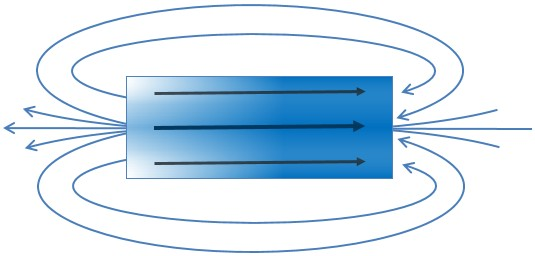
\includegraphics[scale=.7]{sections/images/consciousness_electromaagnetic_force.jpg}
	\floatfoot{Aumento das possibilidades de entrelaçamento de ondas devida a equalização probabilística em objetos próximos e de baixa entropia.}%\footnotemark}
	\end{figure}
	%\footnotetext{Fonte: note}

A Figura \ref{fig:consciousness_electromaagnetic_force_entropy} mostra um exemplo de baixa entropia. 
	\begin{figure}[H]
	\caption{Força eletromagnética - entropia}
	\label{fig:consciousness_electromaagnetic_force_entropy}
	\centering
	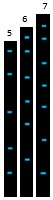
\includegraphics[scale=.9]{sections/images/consciousness_electromaagnetic_force_entropy.jpg}
	\floatfoot{Aumento das possibilidades de entrelaçamento de ondas devido à baixa entropia.}%\footnotemark}
	\end{figure}
	%\footnotetext{Fonte: note}

O aspecto eletromagnético está intimamente relacionado com a baixa entropia de um intervalo e a possibilidade de entrelaçamento de seus pares com os pares ao redor. A baixa entropia de um intervalo indica que suas amostras estão em uma ordem qualquer em seu interior.

Probabilisticamente, os pares de ondas mais parecidos estão nas regiões mais próximas (linhas azuis do Figura \ref{fig:consciousness_electromaagnetic_force}). Isso ocorre devido ao crescimento do número de amostras sentido a mediana da população, porém não é regra e os polos podem se inverter, ou seja, ter mais ligações com a região de menor probabilidade, ainda que a maior parte dos pares que compõem essa região estejam de forma crescente sentido a mediana.

\subsubsubsection{força nuclear}
Os mesmos aspectos probabilísticos que regem a gravidade e que podem ser vistos nas Figuras \ref{fig:consciousness_gravitational_force} e \ref{fig:consciousness_gravitational_force_system} também regem as chamadas forças nucleares. A diferença é que nas forças nucleares os intervalos são menores possibilitando uma quantidade muito maior de saltos e suas ondas são mais discrepantes, conforme mostra a Figura \ref{fig:consciousness_space_subconsciousness_min}.

As forças nucleares forte e fraca representam grandes concentrações de momentos lógicos por intervalo populacional, uma alta densidade em um pequeno intervalo. A grande concentração dessas amostras está no pico do intervalo, que ocupa um subintervalo cada vez menor dentro da onda, devido à alta concentração de amostras em intervalos cada vez menores. Esses picos diminuem proporcionalmente à medida que concentram ainda mais novas amostras. Estes momentos ou amostras tendem a estarem cada vez mais juntos dentro do intervalo formando picos cada vez mais altos e densos. Esses picos são frequentemente encontrados do meio para frente dos sistemas (o núcleo ou pico do sistema), como mostrado na onda mais alta do nível dois da Figura \ref{fig:consciousness_gravitational_force_system}.

A penetração desses intervalos pequenos e densos por uma quantidade excessiva de momentos lógicos (outro intervalo semelhante), em um curto período, faz com que os inúmeros pares desses intervalos (subintervalos) se tornem muito maiores progressivamente. Dessa forma cada subintervalo salta de forma continua, progressiva e rapidamente para correspondentes cada vez maiores até que a probabilidade de destruição normalize todo o intervalo posteriormente.

\subsubsection{Matéria escura e energia escura}


\subsubsection{Antimatéria}
Quando um intervalo tende a concentrar suas amostras sentido da mediana, o que é o sentido provável conforme teorema central do limite, dá-se o nome de matéria. A antimatéria é o contrário, quando um intervalo tende a concentrar suas amostras no sentido oposto à mediana. 

A maneira mais simples de visualizar o sentido probabilístico das amostras de qualquer comprimento de onda é observar a \textbf{linha de referência probabilística}, conforme exibido na Figura \ref{fig:consciousness_space_spiral_reference_line}. Quanto maior a quantidade de amostra de um intervalo maior será sua tendência probabilística sentido a mediana da população.

Na Figura \ref{fig:consciousness_concentration_of_opposite_samples} é exibido dois intervalos idênticos com suas amostras em concentrações opostas.
	\begin{figure}[H]
	\caption{Parte de um intervalo idêntico com suas concentrações de amostras opostas}
	\label{fig:consciousness_concentration_of_opposite_samples}
	\centering
	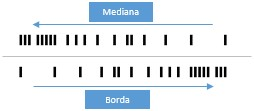
\includegraphics[scale=1.2]{sections/images/consciousness_concentration_of_opposite_samples.jpg}
	\floatfoot{Parte de um intervalo idêntico distribuídos de formas opostas.}%\footnotemark}
	\end{figure}
	%\footnotetext{Fonte: note}

O merge ou soma dos intervalos opostos da Figura \ref{fig:consciousness_concentration_of_opposite_samples} os tornaria um intervalo simétrico, ou seja, não estaria em nenhum dos sentidos.
Na Figura \ref{fig:consciousness_concentration_of_opposite_samples_within_range} é exibido uma população com suas concentrações de amostras sentido à mediana e outra com suas concentrações sentido às bordas do intervalo.
	\begin{figure}[H]
	\caption{Populações com suas concentrações de amostras opostas}
	\label{fig:consciousness_concentration_of_opposite_samples_within_range}
	\centering
	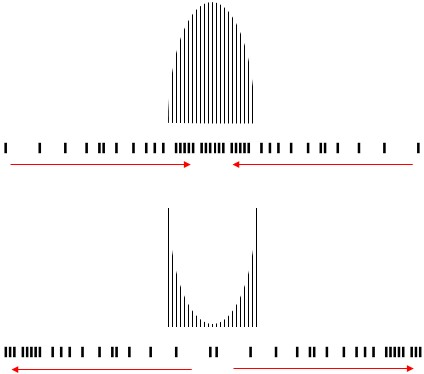
\includegraphics[scale=.7]{sections/images/consciousness_concentration_of_opposite_samples_within_range.jpg}
	\floatfoot{Populações distribuídas em sentidos contrários.}%\footnotemark}
	\end{figure}
	%\footnotetext{Fonte: note}

\subsubsection{Buraco negro}
Os buracos negros são oriundos de um aspecto probabilístico presente em qualquer intervalo da população. Esse aspecto é a alta concentração probabilísticas de amostras em intervalos cada vez menores de uma onda. O pico irá ocupar um subintervalo proporcional cada vez menor dentro do intervalo da onda, mesmo com uma concentração de amostras crescentes. Esses picos são frequentemente encontrados do meio para frente de um intervalo ou sistema (o núcleo ou pico do sistema).

\subsubsection{Observador e a vida}
Os intervalos de ondas (comprimentos de ondas) que uma subconsciência (sub-lógica) é capaz de observar depende do comprimento de ondas que a própria subconsciência é constituída. Dentre todas as possibilidades de intervalos ou comprimento de ondas permitidos por uma população, o observador está em um deles.

A capacidade de comparar ou distinguir a ordem das mudanças de uma sequência amostral é a capacidade lógica de um observador, o observador do tempo (passado e presente). A velocidade dessa observação é dada pelo range que o observador é capaz de comparar, ou seja, o qual rápido ele for capaz de distinguir pequenas mudanças (poucas amostras) o fará perceber que mudanças maiores levam mais tempo (muitas amostras). 

A capacidade lógica de fazer prospecções probabilísticas, dentro das limitações lógicas do observador e com base na probabilidade da distribuição do intervalo ou subintervalo observado é a essência do pensamento e, portanto, da vida. Essas prospecções estão fundamentadas na probabilidade de distribuição de cada intervalo (no sentido do intervalo) e, portanto, estão relacionadas com a detecção de padrão e com possibilidades probabilísticas futuras.

A capacidade de comparar ou distinguir ondas lógicas, subconjuntos ou subconsciências, é a capacidade que define o sujeito (eu). A razoabilidade dessa definição depende da proporcionalidade dessa capacidade de comparação.

A vida \underline{NÃO É}, como qualquer outra lógica. Comumente, as formas mais notáveis de vida se multiplica por estarem na média probabilística do intervalo entre seus picos e vales, por mais diferente que sejam. Porém, algo muito discrepante ou diferente do padrão médio do intervalo tende a não multiplicar e permanecer.

\subsubsubsection{Sentidos}
A parte cognitiva de uma onda não observa a si mesmo diretamente e sim o exterior (a consciência – o todo) ou mais comumente uma parte dela (a subconsciência). Essa observação pode incluir o restante da onda a qual a parte cognitiva faz parte, que também é exterior da parte cognitiva e, portanto, uma subconsciência - parte da consciência. A parte cognitiva da subconsciência humana é, provavelmente, onde se tem o maior pico de ondas do subconjunto humano. Esse é o local onde é observado a maior intensidade de mudanças. Essas mudanças são caracterizadas pelo pensamento (observação e prospecção probabilística de um intervalo) que tende ao infinito (respeitando as limitações lógicas do observador), assim como a essência da lógica, o \underline{NÃO SER}. Ou seja, a parte cognitiva é a parte que está mais próxima da observação do todo, da lógica em sua essência e totalidade, da consciência.

A obtenção de amostras pelos sentidos dos seres humanos os modifica e essas ondulações funcionam como ajustes ou configurações. Cada sentido observa a população amostral de forma independente, como canais de frequências distintos. Assim a visão pode estar vendo objetos muito distantes e os ouvidos escutando sons bem próximos. Os sentidos são limitados pelas ondas que constituem o observador e sua capacidade máxima de observação está limitada na profundidade máxima de intervalos aninhados observados.

Uma característica importante do processo de observação de pequenos intervalos é que eles podem ser observados com partículas ou ondas. Na observação como partícula o observador acompanha um intervalo representado por um par entrelaçado, observando sua forma e movimento consistentes no espaço. No efeito partícula, a consistência da forma e seus movimentos são estabelecidas pelo par entrelaçado, visto que o salto ocorre em um lado do par de cada vez, garantido estabilidade nas mudanças. No intervalo observado como onda o observador acompanha uma das partes que compõe o par entrelaçado observando seus movimentos e saltos, uma vez que os saltos são frequentes em pequenos intervalos.

Talvez não seja possível observar o efeito onda sem entrelaçar seu par. A alta frequência desse intervalo faz com que ele ocupe ou transite rapidamente em uma área ao seu redor, o que pode facilitar o colapso da onda em um ponto especifico e então observar o seu efeito partícula (semelhante ao olho humano) ou em um local mais amplo e observar seu efeito onda com o colapso de muitas amostragens.
